% ============================================================
% Operator-aware support detector pipeline.
% Standalone build:   pdflatex fig_pipeline.tex
% Or include with:    \input{fig_pipeline_body.tex}  in the abstract.
% ============================================================

\documentclass[border=4pt]{standalone}
\usepackage{amsmath, amssymb}
\usepackage{tikz}
\usetikzlibrary{positioning, arrows.meta, fit, backgrounds, calc}

\begin{document}

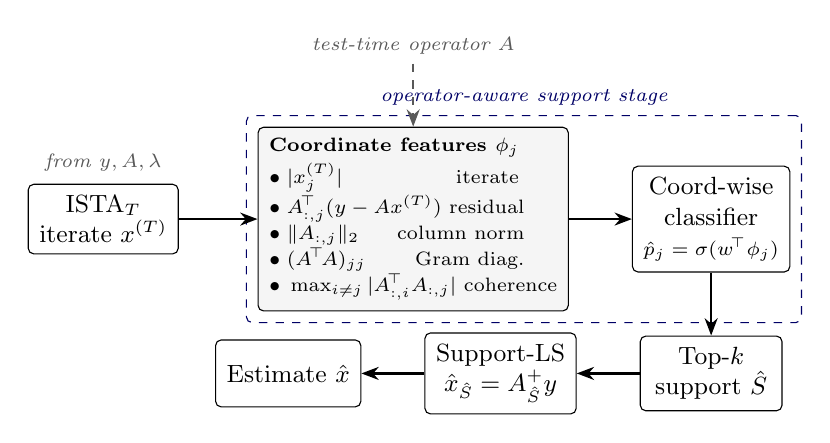
\begin{tikzpicture}[
    font=\small,
    >={Stealth[length=2.2mm]},
    block/.style={
        draw, rounded corners=2pt, align=center,
        inner sep=4pt, minimum height=8.5mm, minimum width=18mm,
        fill=white,
    },
    feat/.style={
        draw, rounded corners=2pt, align=left,
        inner sep=4pt, font=\scriptsize, fill=gray!8,
    },
    src/.style={font=\scriptsize\itshape, gray!70!black},
    arr/.style={->, thick},
]

% --- Inputs -------------------------------------------------
\node[block] (ista) {ISTA$_T$ \\ iterate $x^{(T)}$};
\node[src, above=0.3mm of ista] {from $y, A, \lambda$};

% --- Feature vector phi_j ----------------------------------
\node[feat, right=10mm of ista] (phi) {
    \textbf{Coordinate features $\phi_j$} \\[1pt]
    $\bullet\; |x^{(T)}_j|$ \hfill {\scriptsize iterate} \\
    $\bullet\; A_{:,j}^{\!\top}(y - A x^{(T)})$ \hfill {\scriptsize residual} \\
    $\bullet\; \|A_{:,j}\|_2$ \hfill {\scriptsize column norm} \\
    $\bullet\; (A^{\!\top}\!A)_{jj}$ \hfill {\scriptsize Gram diag.} \\
    $\bullet\; \max_{i\neq j} |A_{:,i}^{\!\top} A_{:,j}|$ \hfill {\scriptsize coherence}
};

% --- Classifier --------------------------------------------
\node[block, right=8mm of phi] (clf)
    {Coord-wise \\ classifier \\ \scriptsize $\hat p_j = \sigma(w^{\!\top}\phi_j)$};

% --- Top-k support -----------------------------------------
\node[block, below=8mm of clf] (topk)
    {Top-$k$ \\ support $\hat S$};

% --- Least squares -----------------------------------------
\node[block, left=8mm of topk] (ls)
    {Support-LS \\ $\hat x_{\hat S} = A_{\hat S}^{+} y$};

% --- Output ------------------------------------------------
\node[block, left=8mm of ls] (out) {Estimate $\hat x$};

% --- Arrows ------------------------------------------------
\draw[arr] (ista) -- (phi);
\draw[arr] (phi) -- (clf);
\draw[arr] (clf) -- (topk);
\draw[arr] (topk) -- (ls);
\draw[arr] (ls) -- (out);

% --- Test-time operator side-channel into phi --------------
\node[src, above=8mm of phi.north] (Aside)
    {test-time operator $A$};
\draw[arr, dashed, gray!70!black] (Aside) -- (phi.north);

% --- Bracket: "operator-aware" features --------------------
\begin{scope}[on background layer]
\node[draw=blue!40!black, dashed, rounded corners=2pt,
      fit=(phi)(clf), inner sep=4pt, label={[font=\scriptsize\itshape, blue!40!black]above:operator-aware support stage}] {};
\end{scope}

\end{tikzpicture}

\end{document}
